\subsection{Создание механизма восстановления движения по акселерометру и гироскопу (Самарин Артем)}

В этой части задачей было научиться восстанавливать движения телефона по имеющимся у нас данным – времени, показателям акселерометра и гироскопа.

\subsubsection{Неудачный способ}

Для начала задача решалась самым прямым образом - данные акселерометра (т.е. ускорение по каждой из осей телефона) дважды интегрировались и таким образом получалось положение телефона в каждый момент времени, но из-за большой погрешности, двойного интегрирования и помех ничего не вышло – картинка съезжала и вместо, допустим, нужного нам квадрата, получалась спираль. Изначально, это списывалось на то, что акселерометр учитывает ускорение свободного падения, но это оказалось не так – оказалось, что многое зависит от телефона, на котором проводятся измерения, но ещё больше зависит от угла поворота телефона и погрешности при двойном интегрировании.

\subsubsection{С чем вообще работаем?}

На вход я получаю уже отфильтрованный массив с 7-ю параметрами: время от начала движения, ускорение по оси X, ускорение по оси Y, ускорение по оси Z, угол поворота в радианах по X (Pitch), по Y (Roll) и по Z (Yaw).

\begin{figure}[H]
    \center{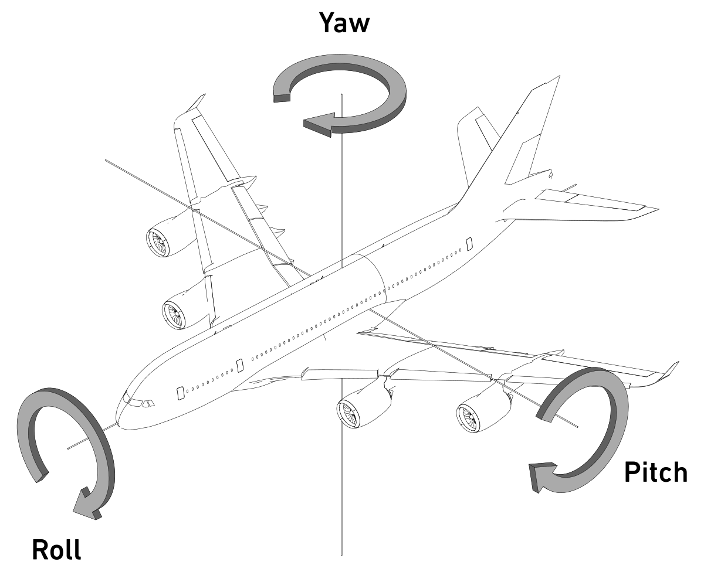
\includegraphics[scale = 0.7]{sam_images/1.png}}
\end{figure}

\subsubsection{Нормализация данных}
Хоть данные уже и отфильтрованы другим членом моей команды – я, для того, чтобы 3D изображение фигур получалось более гладким, использую дополнительный, но очень простой, фильтр:

\begin{figure}[H]
    \center{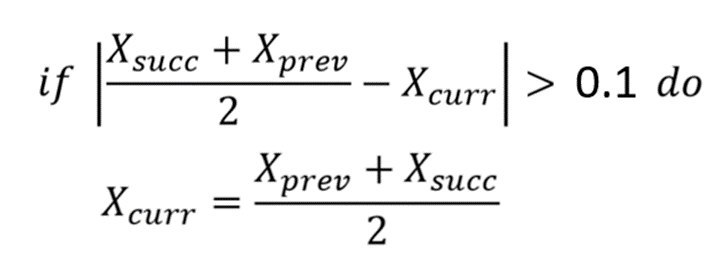
\includegraphics[scale = 0.7]{sam_images/2.jpeg}}
\end{figure}

данные не не искажались по какой-нибудь одной оси – из каждого вектора данных акселерометра вычитается среденее по этому вектору.

\begin{figure}[H]
    \begin{center}
        \begin{tabular}{cc}
            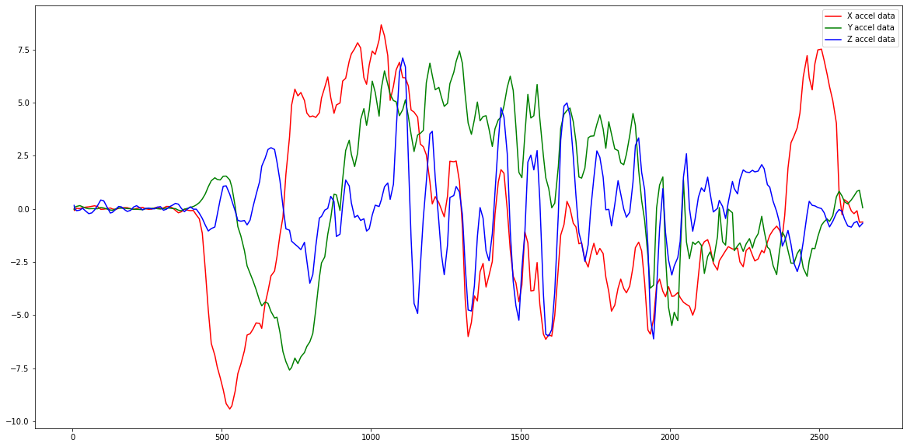
\includegraphics[width=0.45\textwidth]{sam_images/graph_1.png} & 
            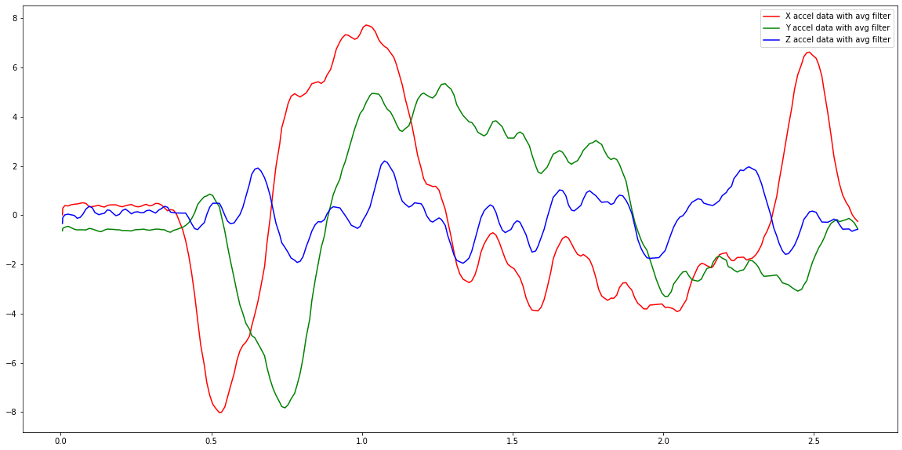
\includegraphics[width=0.45\textwidth]{sam_images/graph_2.png} \\
        \end{tabular}
    \end{center}
    \caption{Рис. 1: Голые и нормализованные данные.}
\end{figure}

\subsubsection{Нахождение положения телефона без учета данных из гироскопа}

После того как данные нормализованы – как уже говорилось ранее – данные акселерометра дважды интегрируются. Если данные акселерометра по X – это вектор А, а время – это вектор T, то положение в каждый момент времени определяется, как $A[i] * (T[i] - T[i-1])$.

\begin{figure}[H]
    \begin{center}
        \begin{tabular}{cc}
            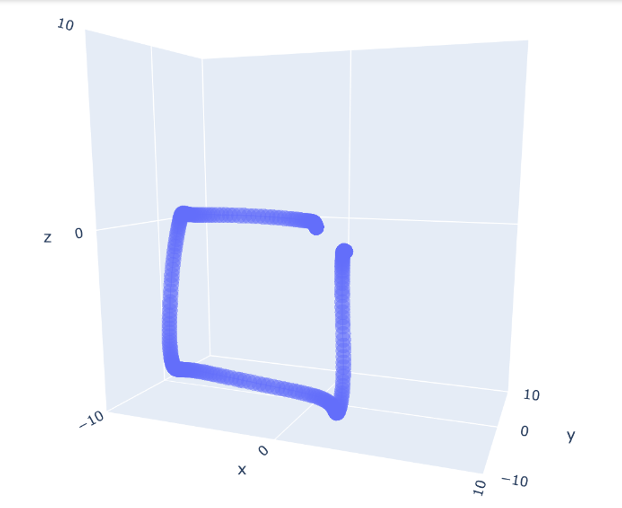
\includegraphics[width=0.45\textwidth]{sam_images/3d_graph_1.png} & 
            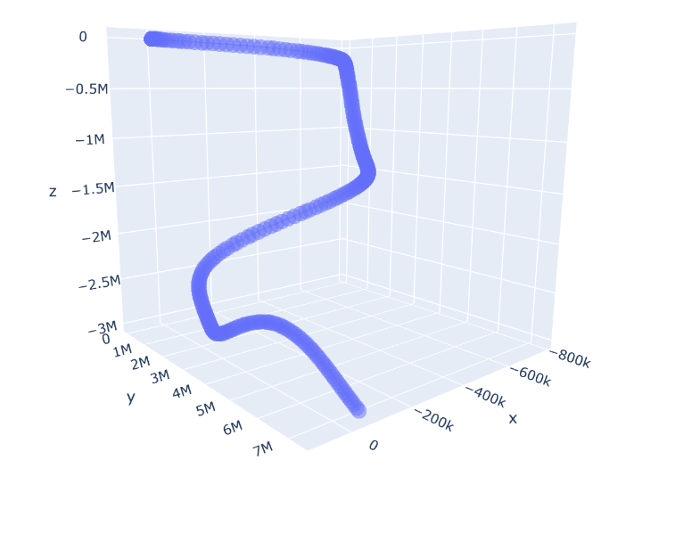
\includegraphics[width=0.45\textwidth]{sam_images/3d_graph_2.png} \\
        \end{tabular}
    \end{center}
    \caption{Рис. 2: Квадрат в 3D до фильтрации и нормализации данных и после.}
\end{figure}

\subsubsection{Почему и как это работает?}

Когда человек рисует жест (а это основной смысл разрабатываемой нами технологии), то он стоит на месте и телефон, как правило, держит в одном положении, просто потому что это удобно – телефоны широкие и как либо менять угол его поворота сложно, если не делать это намеренно. Соответственно, если угол поворота телефона меняется, то хорошее отображение движения телефона не получится.
\newpage

\subsubsection{Как и зачем учитывать данные гироскопа?}

Данные гироскопа учитываются для того, чтобы компенсировать угол вращения телефона. Если учитывать угол поворота, то можно получить положение телефона относительно земли, а не относительно движения вдоль своих осей. Для этого берется вектор углов относительно земли в момент времени i, вычисляется матрица поворота вокруг произвольного угла (указана ниже) и умножается на вектор показаний акселерометра в тот же момент времени i. Таким образом, мы можем компенсировать вращение телефона во время движения и находить более точное положение телефона в пространстве при последующем интегрировании.

\begin{equation*}
    \begin{pmatrix}
        cos(z)*cos(y) & -sin(z)*cos(x) + cos(z)*sin(x)*sin(y) & sin(z)*sin(x)+ cos(x)*cos(z)*sin(y) \\
        cos(z)*cos(y) & cos(z)*cos(x) + sin(x)*sin(y) & -cos(z)*sin(x)+ cos(x)*sin(z)*sin(y) \\
        -sin(y) & cos(y)*sin(x) & cos(x)*cos(y) \\
    \end{pmatrix}
\end{equation*}

\begin{figure}[H]
    \begin{center}
        \begin{tabular}{cc}
            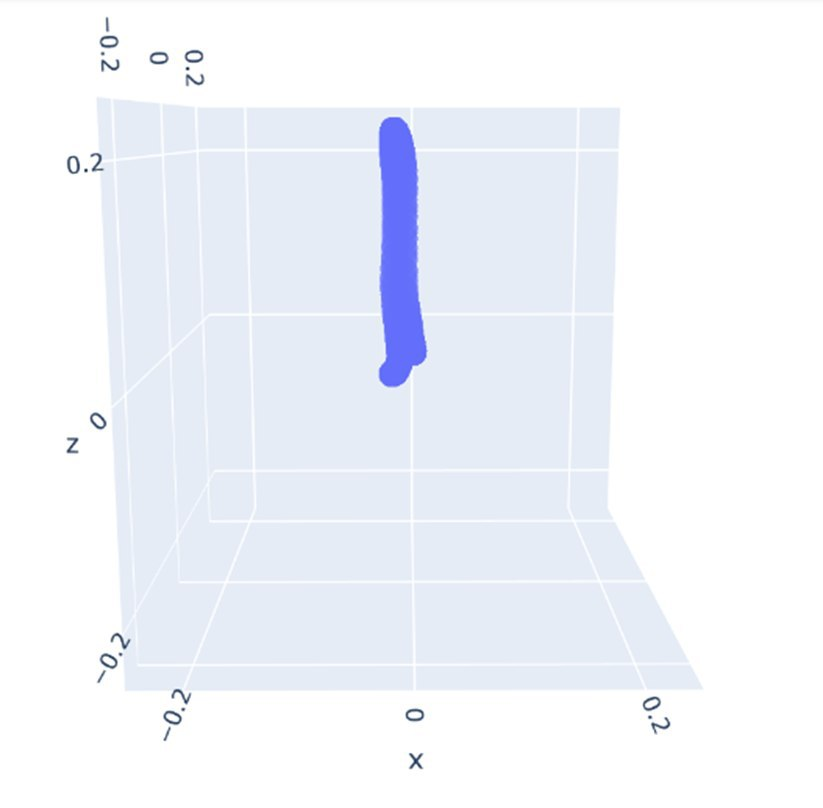
\includegraphics[width=0.45\textwidth]{sam_images/last_1.jpeg} & 
            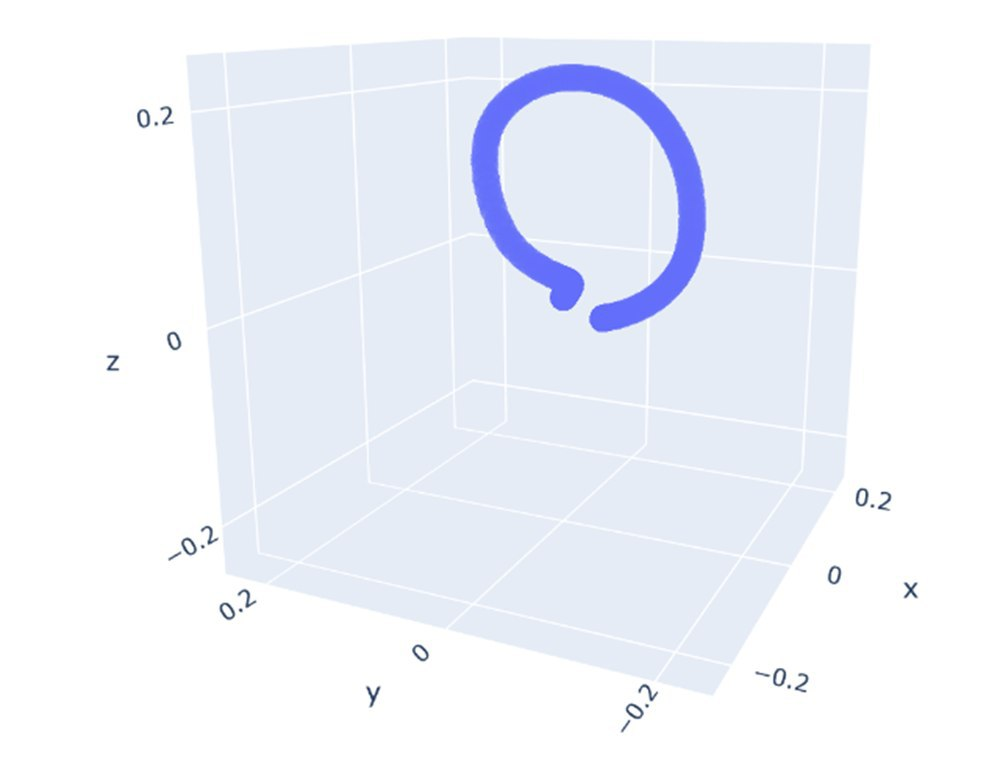
\includegraphics[width=0.45\textwidth]{sam_images/last_2.jpeg} \\
        \end{tabular}
    \end{center}
    \caption{Рис. 3: Круг с учетом всех данных и фильтров.}
\end{figure}